\documentclass[a4paper]{article}
\usepackage[utf8]{inputenc}
\usepackage[english]{babel}
\usepackage[hidelinks]{hyperref} 
\usepackage{biblatex}
\usepackage{csquotes}
\usepackage{amssymb}
\usepackage{amsmath}
\usepackage{mathtools}
\usepackage{graphicx}
\usepackage{float}
\usepackage{listings}
\usepackage{xcolor}

\graphicspath{{./figures/} }

\addbibresource{documentation.bib}

\DeclareMathOperator*{\argf}{argf}
\DeclareMathOperator*{\argmin}{argmin}
\DeclareMathOperator*{\VT}{\textit{VT}}

\definecolor{codegreen}{rgb}{0,0.6,0}
\definecolor{codepurple}{rgb}{0.6,0,0.8}
 
\lstdefinestyle{output}{
	basicstyle=\ttfamily,
	numbers=none
}
 
\lstdefinestyle{python_code}{
    keywordstyle=\color{codepurple},
    stringstyle=\color{codegreen},
	basicstyle=\ttfamily,
	numbers=left, 
	numberstyle=\ttfamily\footnotesize
}

\title{A Python interface for weighted Voronoi Tessellations in the Euclidean plane}
\author{Lucas Fein}

\begin{document}
\maketitle
\vfill
\tableofcontents
\begin{center}
	The code of the interface presented here, this documentation, as well as the code used to produce figures and listings
	for this documentation is available at
	\href{https://github.com/lucasfein/voronoi}{\texttt{https://github.com/lucasfein/voronoi}}
\end{center}
\thispagestyle{empty}
\pagebreak

\setcounter{page}{1}
\section{Introduction}
The objective of the internship was to implement an efficient interface for the creation of and examination of
weighted Voronoi Tessellations as a model for cell layer morphology. This is particularly interesting as,
due to the selective staining techniques, footage of cell layers often cover either cell nuclei, or membranes,
the latter of which Voronoi Tessellations may provide an assumption for that is compatible with work in the
field of force inference models of biological tissues.

Despite disputable biological accuracy of straight cell membranes,
motivating for example \cite{Bock2010}, the assumption is common in models of force-inference, such as \cite{Ischihara2012}.

\section{Voronoi Tessellation}
A Voronoi Tessellation is a partitioning of a metric space \(S = (M, d)\) based on a subset of elements
referred to as generators \(G \subseteq M\).
It associates each element \(p \in M\) with any one generator optimizing a particular relationship between
\(p\) and \(G\) given the metric \(d\),
such that the set of elements associated with any generator \(N(g'), g' \in G\), referred to as its neighborhood,
is given by \[N(g') = \{p \in M \,|\, \argf_{G} (d(g, p)) = \{g'\}\}\]

The most common instance of the Voronoi Tessellation is a planar map of proximity,
i.e. the metric space is given as the Euclidean plane \(S \coloneqq (\mathbb{R}^2, d_e)\) where \(d_e\)
is the Euclidean distance and the distances between generators and the elements in their neighborhood are minimized,
formally \(\argf := \argmin\).

The partitioning obtained from a Voronoi Tessellation is represented employing points which are equidistant to multiple
generators and therefore form the boundaries of adjacent neighborhoods. In the Euclidean plane this results in a specific
embedding of an undirected planar graph \(\VT(S, G, \argmin) = (V, E)\) which may be defined as
\[V \coloneqq \{p \in \mathbb{R}^2 \,|\, |\argmin_{G} (d_e(g, p))| \geq 3\}\]
\[E \coloneqq  \{\{p, q\} \subset V \,|\, |\argmin_{G} (d_e(g, p)) \cap \argmin_{G} (d_e(g, q))| = 2\}\]
for representing proximity.

\begin{figure}[H]
	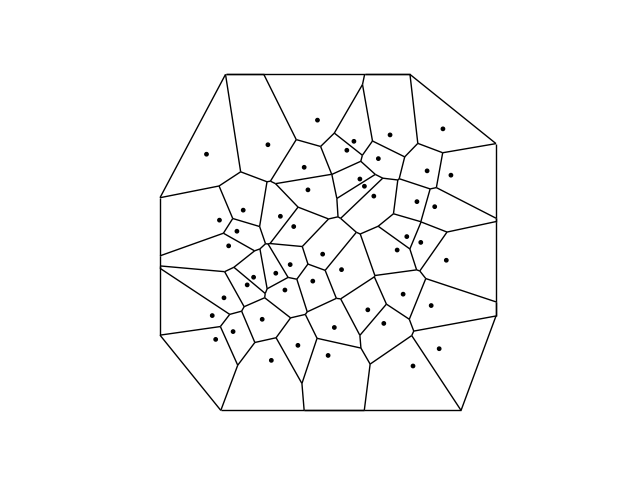
\includegraphics[width=\textwidth]{voronoi_tessellation.png}
	\caption{The bounded Voronoi Tessellation resulting from a set of generators.}
\end{figure}

The edges of the graph divide the plane into which it is embedded into the individual neighborhoods of each generator,
each edge separating two adjacent regions. These regions correspond to subsets of the metric space.

The boundary is established by allowing each edge to extend until the limits of the given plane and connecting the
resulting endpoints. While it violates the formal definition of a Voronoi Tessellation, as some points are falsely
excluded from neighborhoods, it serves the purpose of associating each generator with a bounded face. This
is important for generator approximation.

\subsection{Computation using the Delaunay Triangulation}
The approach presented in the following applies to nearest-point Voronoi Tessellations in the Euclidean plane, therefore
\(\VT(G) := \VT((\mathbb{R}^2, d_e), G, \argmin)\) with \(G \subseteq \mathbb{R}^2\).

A Delaunay Triangulation \(DT\) is a tessellation using triangles given a set of points, such as the generators \(G\).
These triangles are composed from the vertices in such a way that there is no triangle
containing any generator \(g \in G\) inside its circumcircle, i.e. the circle uniquely determined by
the three vertices of the triangle. These are, placed on the circumcircles circumference,
equidistant to its center, the circumcenter.

Employing the Bowyer-Watson-Algorithm the Delaunay Triangulation of a set of generators \(DT(G)\) can,
be computed in \(\mathcal{O}(m^2))\), \(m\) being the number of generators.

Starting from a triangle enclosing
the entire area that generators are placed in, the algorithm works incrementally
by considering one generator in each iteration \(i \in \{1 \cdots |G|\}\) and repartitioning the current
triangulation in order to restore the decisive property of the Delaunay Triangulation. When a generator \(g_i\) is added,
each triangle of the current
triangulation is examined in order to determine which triangles' circumcenters contain \(g_i\), i.e. no longer
fulfill the property of the Delaunay Triangulation given the updated set of generators. By determining the shared
edges of the incompliant triangles and removing them the outer edges of these triangles remain, forming a
polygon. By constructing triangles between each edge of this polygon and \(g_i\), compliant triangles are created.
This means that after the \(i\)th iteration the Delaunay Triangulation is valid for a subset of \(i\)
generators.

A Voronoi Tessellation can be obtained relatively easily from a Delaunay Triangulation
in \(\mathcal{O}(n^2))\), \(n\) being the number of triangles of the Delaunay Triangulation.
The circumcenters of the triangles of Delaunay Triangulation resemble a set of vertices
to which three generators are equidistant, yielding the set of vertices \(V\) of a
Voronoi Tessellation. The circumcenter of a triangle is determined as the intersection of the perpendicular bisectors
of the triangle edges. If two generators are equidistant to the same two circumcenters,
the triangles implying these circumcenters share a common edge. The perpendicular bisector to this edge,
drawn between both circumcenters resembles an edge of the Voronoi Tessellation, separating two neighborhoods.

Edges that are not common to any other triangle
indicate adjacent neighborhoods at the periphery of the set of generators.
These are separated by the perpendicular bisector of this edge starting from the circumcenter of the triangle
that the edge belongs to.

\begin{figure}[H]
	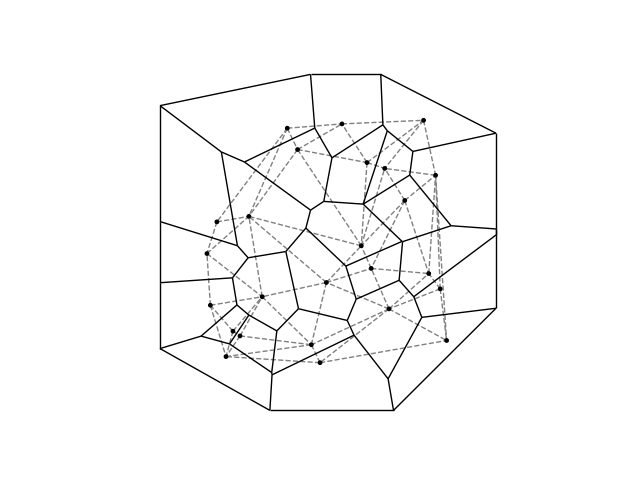
\includegraphics[width=\textwidth]{delaunay_triangulation.png}
	\caption{The dashed line indicates the Voronoi Tessellations' underlying Delaunay Triangulation.}
\end{figure}

Formally, a Voronoi Tessellation is the dual of a Delaunay Triangulation and vice versa. Each face of the
Voronoi Diagram, results from a generator, a vertex of the Delaunay Triangulation and each triangular
face of the Delaunay Triangulation provides a circumcenter, a vertex of the Voronoi Tessellation.

\subsection{Generator weights}
A Voronoi Tessellation may be extended by assigning weights \(w(g) \in \mathbb{R}\) to the generators and
extending the metric \(d\) accordingly. Most commonly this is achieved by subtracting it.
\[d_w(g, p) \coloneqq \max(\{0, d(g, p) - w(g)\})\]
This results in a circular region with a radius of \(w(g)\) around the generator \(g\)
that is excluded from the partitioned space, making it an \(n\)-dimensional sphere in \(\mathbb{R}^n\).
The distance to any point is effectively measured not from the circles' center, the generator,
but the closest point on the circles' circumference to any \(p\).
Weighted generators in the plane are commonly referred to as disks.

\begin{figure}[H]
	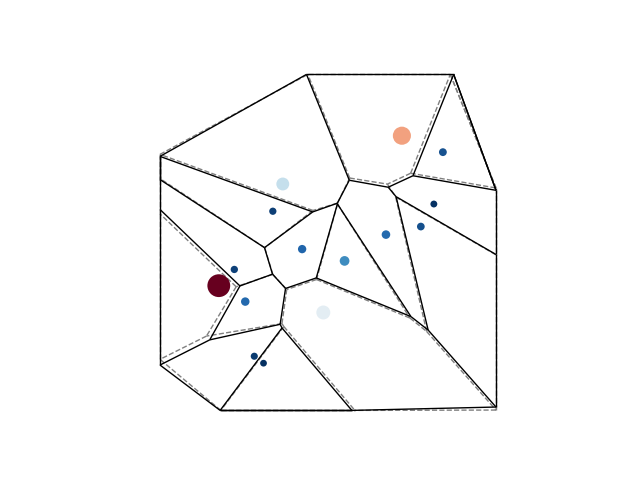
\includegraphics[width=\textwidth]{generator_weights.png}
	\caption{The effect of different generator weights. The gray dashed line indicates the diagram resulting from
		uniformly weighted generators. Blue indicates a relatively small, red a relatively large generator with respect
		to the range of weights.}
\end{figure}

In order to shift the circumcenter of each triangle to account for the weight difference between any two generators
it is shifted by the mean of three vectors, each generated from one edge of a triangle.
Each edge of a triangle between any two  of its points resembles a vector between these points with the orientation
of that edge. The vector between these generators is scaled by the signed weight difference relative to its entire length.

Should the proposed shift be longer than the distance to the nearest circumcenter, it will be ignored
in order to avoid potential overlaps.

\subsection{Generalization}
In \cite{Bock2010} the authors propose a generalization of Voronoi Tessellations generating a morphology
widely similar to that of keratinocytes in epithelial cell layers by generating curved boundaries of adjacent cells.
Formally, this is achieved by extending the metric with division of \(d_e(g, p)\) by the squared generator weight
\(w(g), g \in G\). For any \(g\) and \(p \in \mathbb{R}^2\) the distance \(d_c\) is given as:

\[d_c(g, p) := \frac{d_e(g, p)^2}{w(g)^2}\]

It was attempted to implement this instance of the Voronoi Tessellation, however several problems remain.
The implementation presented in the following is based on example tessellations in the respective publication.

\begin{figure}[H]
	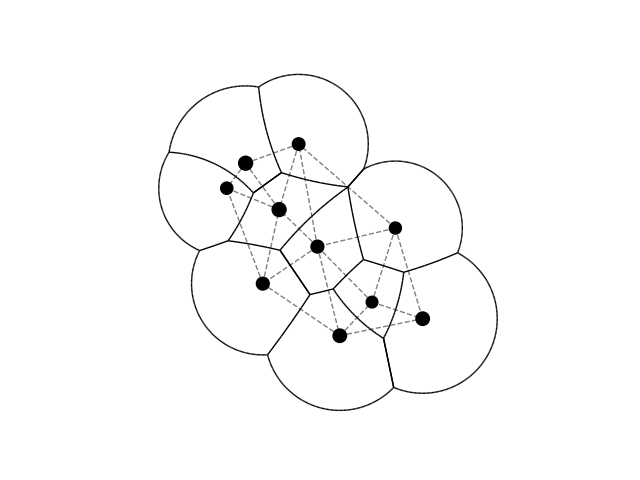
\includegraphics[width=\textwidth]{circular_voronoi_tessellation.png}
	\caption{A circular Voronoi Tessellation according to \cite{Bock2010} and its underlying Delaunay Triangulation}
\end{figure}

Similar to the computation of the Voronoi Tessellation previously introduced, the Delaunay Triangulation is
employed to determine the boundary of adjacent neighborhoods. Each edge of the Delaunay Triangulation
generates a circular boundary \(c_{ij}\) based on the difference of weights between two generators \(g_i, g_j \in G\), the
curvature being proportional to the differences' absolute value, since the radius \(r_{ij}\) of the circle is given as:

\[r_{ij} := \frac{w(g_i)w(g_j)}{(w(g_i)^2 - w(g_j)^2)}d_e(g_i, g_j)\]

The intersections of the three circles resulting from each edge of a triangle of the Delaunay Triangulation
resemble the vertices of the Voronoi Tessellation. They are analogous but not identical to the circumcenters of
the Delaunay Triangulation and are located close to the respective triangles' centers.

The curved boundaries result from partial circles defined between the intersections
of the triangles of the Delaunay Triangulation that share an edge.

The curved closure of the diagram
is derived from circles centered around the generators with radii resulting from uniformly
scaling the weight of any generator \(w(g), g \in G\) at the boundary by a constant factor \(s \in \mathbb{R}\).
Partial sections between the intersections resulting from these circles determine the closure.

This results in an extended definition of \(N(g)\):

\[N(g) := \{p \in M \,|\, \argf_{G} (d_c(g, p)) = \{g\} \land d_c(g, p) \leq sw(g)\}\]

\section{Generator approximation}
In the following, only nearest-point Voronoi Tessellations in the Euclidean plane are considered, therefore
\(\VT(G) := \VT((\mathbb{R}^2, d_e), G, \argmin)\) with \(G \subseteq \mathbb{R}^2\).

Given the fact, that a Voronoi Tessellation can be uniquely determined from a set of generators, it appears as
an interesting question, whether the opposite can be achieved easily. In order to approximate generators that yield
a Voronoi Tessellation that resembles the original as closely as possible a regression was implemented.

The approach translates approximated generators in order to minimize the mean deviation between the closest vertices of the
Voronoi Tessellation resulting from the approximated generators and the original Voronoi Tessellation.

\subsection{Centroid determination}
In order to achieve a sensible initial state for the regression, the approximated generators are set to the centroids
of the faces of the original Voronoi Tessellation, an embedding of an undirected planar graph.
In order to determine these a variation of Depth-first search is applied,
that was adapted from \cite{Schneider2015}. The search traverses the graph in form of an adjacency matrix,
starting at each vertex.
Along with a current node \(n_i\), each recursion maintains the sequence of nodes it
previously visited \((n_{1}, \dots, n_{i-1})\).
One the first within the sequence  of previously visited nodes is considered as the current node (\(n_i = n_1\))
a cycle in the graph containing \(i-1\) vertices is found.

The search space is minimized by not considering all adjacent vertices given the current vertex but only the
vertex \(n_{i+1}\) such that the counter-clockwise angle between the vectors from \(n_i\) to \(n_{i-1}\) and \(n_{i+1}\),
respectively, is minimized by including information from the graphs' embedding.

In order to assure that all faces saved are unique, it is also necessary to identify redundant faces.
These originate from identifying the same face after starting the recursion at distinct vertices both part of
that face. The removal of redundant faces is achieved by exhaustively comparing faces with similar number of vertices.
One face will be discarded if it shares all vertices with another.

A different consequence of the selective progression is that only cycles are identified
and that all identified cycles, except for one, are chordless, i.e.
there is no edge between any two vertices of a cycle that is not itself part of that cycle.
Such an edge would have a smaller angle. The only non-chordless cycle reported is the one clockwise around the entire
perimeter of the Voronoi Tessellation which can be most reliably identified and discarded by the fact
that its area is the sum of the areas of all other unique faces of the graph.

Given the sequence of vertices forming a non-self-intersecting simple polygon, its area and centroid can be determined
easily and unambiguously as opposed to polygons containing concave areas.

\begin{figure}[H]
	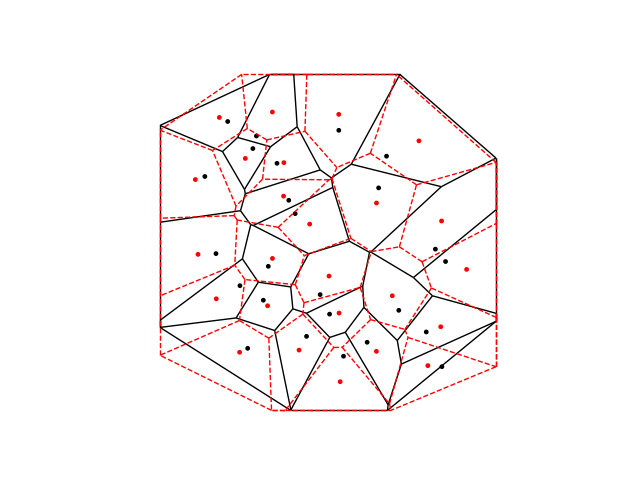
\includegraphics[width=\textwidth]{face_centroids.png}
	\caption{The red dots indicate the centroids of the determined faces. The red dashed line indicates the
		Voronoi Tessellation resulting from the centroids used as generators. \(|G| = 25\)}
\end{figure}

The figure above demonstrates that a generator may be located relatively far away from the centroid of its
own neighborhood. This results in a very different structure of the Voronoi Tessellation obtained from the centroids,
indicating a poor approximation of generators.

However, even in these cases, the number of vertices
of the face forming the original neighborhood and the corresponding face in the approximation are similar,
which motivates an approach to improve the approximation.
\begin{figure}[H]
	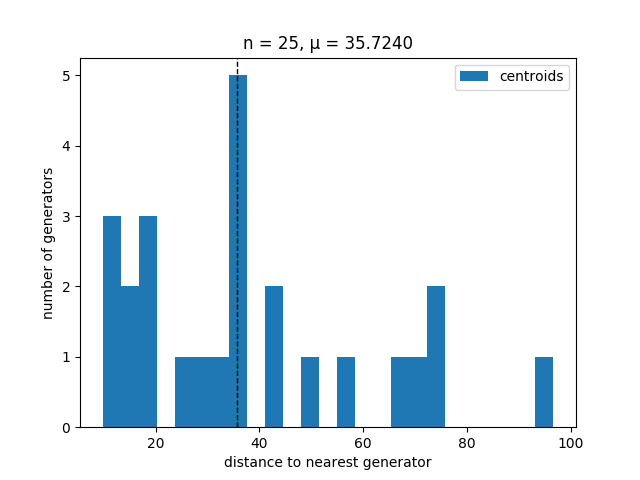
\includegraphics[width=\textwidth]{centroid_distance_histogram.png}
	\caption{The distribution of distance from the neighborhoods' centroid across generators in the previous figure.
		The generators are uniformly weighted. \(\mu\) is the median.}
\end{figure}

\subsection{Improvement of the approximation}
In order to obtain a set of generators that serves as an approximation of the unknown generators \(G\)
of a known Voronoi Tessellation \(\VT(G)\), the approach attempts to determine a set of generators \(\hat{G}\)
that produces a Voronoi Tessellation \(\VT(\hat{G})\) that minimizes the error to \(\VT(G)\). This error is
measured as the mean minimal error between the vertices of \(\VT(G)\) and \(\VT({\hat{G}})\), i.e. the
mean error between the pairs of closest vertices from both sets.

This mapping is injective to reduce
ambiguity, i.e. for \(g \in G\) and \(\hat{g}, \hat{g}' \in \hat{G}\), if \(g\) is the closest generator to both
\(\hat{g}\) and \(\hat{g}^\prime\) but \(d_w(g, \hat{g}) < (d_w(g, \hat{g}^\prime)\), \(\hat{g}^\prime\) 
will not be mapped to \(g\).

In order to achieve this, each generator \(\hat{g} \in \hat{G}\) is shifted by the mean of the vectors that would translate
any one vertex of the face that resembles the neighborhood of \(\hat{g}\), \(N(\hat{g})\) to its closest vertex in
the original Voronoi Tessellation, \(\VT(G)\). Additionally, the weight of \(\hat{g}\) is adjusted according to the ratio of the
areas of the corresponding faces in both Voronoi Tessellations.

The underlying principle of this approach relies on a mapping linking \(\hat{G}\) to the faces of \(\VT(\hat{G})\) and
the faces of \(\VT(\hat{G})\) and \(\VT(G)\). The former is implemented by mapping face centroids to
their closest generator.As \(\hat{G}\) is initially determined as the centroids of the faces of the original
Voronoi Tessellation \(\VT(G)\), the face of \(\VT(G)\) that any approximated generator \(\hat{g} \in \hat{G}\) originates
from is known.

By employing the mean of several shifts, faces of \(\VT(\hat{G})\) that present a mean offset in a particular
direction relative to the corresponding face of \(\VT(G)\) will result in a translation of their associated
generator according to the offset. Faces from \(\VT({\hat{G}})\) which are associated with a smaller or larger
face from \(\VT(G)\) will not cause an approximated generator to translate, but to scale proportionally to the area
of the corresponding face from \(\VT(G)\). In order to emphasize location over weight, the scaling
is bounded to fraction of its neighborhoods' area.

The generators are currently processed in the order of the vector containing them,
which is arbitrary relative to the structure of the  Voronoi Tessellation. The regression seizes once the error can not
be reduced after processing the entire set of generators.

\begin{figure}[H]
	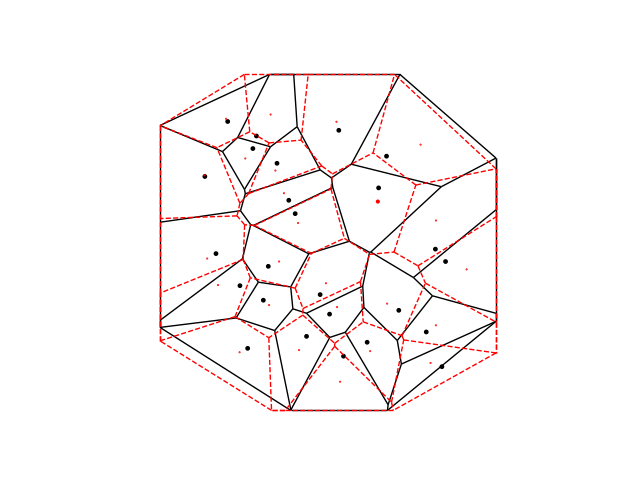
\includegraphics[width=\textwidth]{generator_approximation.png}
	\caption{As previously, red dots indicate approximated generators \(\hat{G}\). The red dashed line indicates
		the resulting Voronoi Tessellation, \(\VT(\hat{G})\), which is employed to determine improvement of the approximation.
		Here generator weights are displayed accurately via the generators' respective radii, since the weight is considered
		during the regression.}
\end{figure}

The above figure presents result of an approximation of a randomized set of generators \(G\).
The edges of the Voronoi Tessellation resulting from the approximated generators, \(\VT(\hat{G})\) appear more accurately placed.
The limitations of the approach are also visible. However, given the measures addressed previously,
in the following, the improvement achieved by the approach in this example shall be quantified.

\begin{figure}[H]
	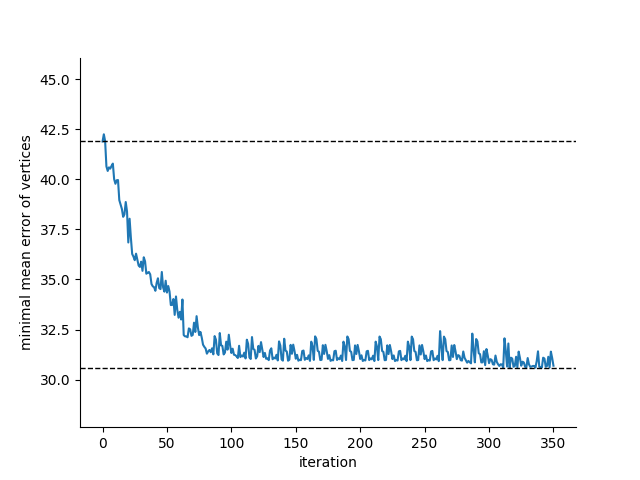
\includegraphics[width=\textwidth]{generator_approximation_error.png}
	\caption{The development of the minimal mean error between the vertices of \(\VT(G)\) and \(\VT(\hat{G})\)
		during regression, which is the observable parameter assumed to indicate improvement of the approximation.
		A Voronoi Tessellation with an updated set of approximate generators \(\hat{G}\),
		\(\VT(\hat{G})\) is determined in each iteration to evaluate the update of \(\hat{G}\).
		The errors resulting from all proposed shifts are displayed, regardless of whether the generator translation
		was  discarded or not.}
\end{figure}

It is visible, that the largest improvement is achieved after about a third of total iterations, suggesting
that a threshold may be applied to terminate the regression
once the improvement of the error is consistently below a threshold \(\epsilon > 0\) and thereby favour speed over accuracy.
However, in the interest of evaluating the regression as precisely as possible, no threshold was used (\(\epsilon = 0\)).
Further, the figure shows that individual proposed translations do not become more favorable over time,
after other translations are made. Instead, the abundant peaks suggest the persisting proposal of a disadvantageous
generator translations.

\begin{figure}[H]
	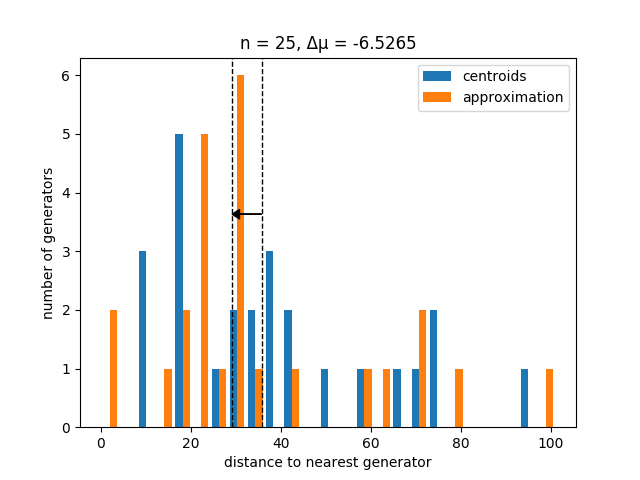
\includegraphics[width=\textwidth]{generator_approximation_histogram.png}
	\caption{The comparison of the initial and final state of the deviation of \(\hat{G}\) and \(G\).
		The median and distribution in general indicate an improvement of the approximation.}
\end{figure}

In the interest of reproducibility the regression is entirely deterministic. However,
as \(G\) is randomized and the improvement achieved by the approximation varies,
the difference of the median error of \(G\) and \(\hat{G}\), denoted as \(\Delta\mu\), is a random variable.
Its distribution is a more general indication of the approaches validity than the single example examined previously.

\begin{figure}[H]
	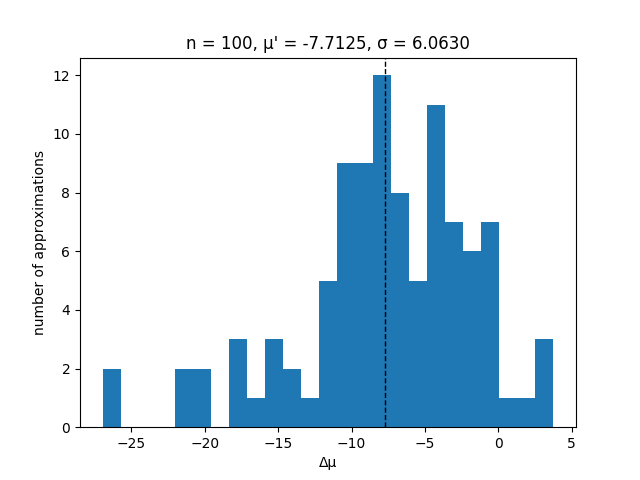
\includegraphics[width=\textwidth]{approximation_improvement.png}
	\caption{The distribution of \(\Delta\mu\) sampled from independent attempts with random \(G\).
		Negative values indicate an improvement of generator approximation \(\hat{G}\) over the face centroids achieved by
		regression. The fact that the distribution extends into positive values, shows that, interestingly,
		\(\Delta\mu\) does not necessarily decrease with the mean error of the vertices of \(\VT(G)\) and
		\(\VT(\hat{G})\), which is being minimized during regression. \(\mu^\prime\) is the mean.}
\end{figure}

This more comprehensive overview demonstrates that the presented approach may be expected to produce an
improvement. However, it is likely not to improve and may yield a worse approximation by measure of the median minimal
distance of \(G\) and \(\hat{G}\) than the face centroids themselves provided initially. In this case, however, a better
approximation being available, one would retain the centroids rather than the result of the regression.

\begin{figure}[H]
	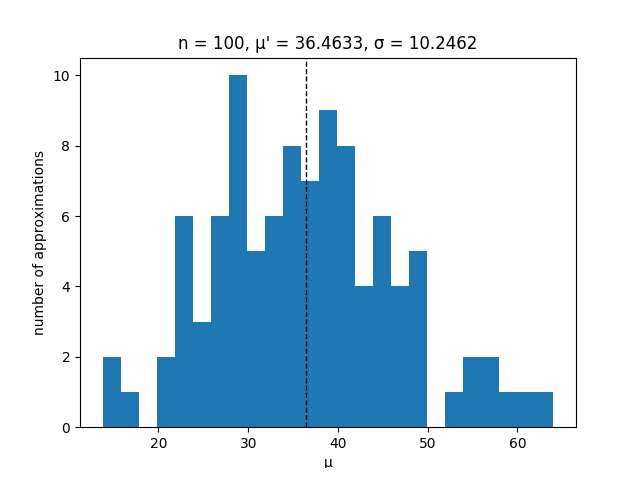
\includegraphics[width=\textwidth]{approximation_performance.png}
	\caption{The distribution of the median error between the closest pairs from \(G \times \hat{G}\),
		chosen between the face centroids and the result of a deterministic attempt of improving the approximation,
		\(\mu^\prime\) is the mean.}
\end{figure}

This distribution shall indicate, rather than the performance of the improvement previously presented itself, the
overall ability of the library to approximate a set of generators \(G\), measured as the median distance between
the closest elements in \(G\) and \(\hat{G}\).

Finally run time of the approach severely increases with the number of generators, \(|G|\). Further,
it is an interesting question how density of the embedding affects the performance of the regression.

\begin{figure}[H]
	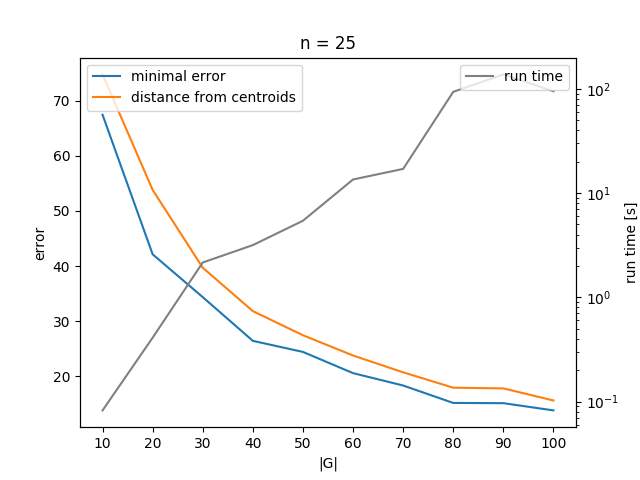
\includegraphics[width=\textwidth]{approximation_generator_density.png}
	\caption{The mean error achieved for variable \(|G|\). Each \(|G|\) was sampled with \(n\) independent runs.
		In order to account for uniformly decreasing distances as a natural result of increased generator density,
		the mean error of the centroids is shown as reference.}
\end{figure}

The difference between the result of the regression and the initial distances of \(G\) and the centroids
reduces slightly for increasing \(|G|\), which suggests that the performance of the approach presented is
slightly decreases with increasing generator density.

\section{Image segmentation}
Since the interface is intended to be used on biological data deriving from footage, image segmentation
appeared as an interesting extension of functionality and its implementation was attempted.

In terms of application to biological data, cell nuclei correspond to the generators.
These are stained using DAPI, resulting in images in which only blue fluorescent cell nuclei are visible.
Given their location an weight, a Voronoi Tessellation resembling the invisible cell membranes can be constructed,
which is suitable approximation in the context of force inference models.

\subsection{Generators}
Segmentation of digital images is simplified by reducing the three available channels for red, green and blue to one.
In the case of DAPI staining, rather than merging the three channels to a grayscale, employing the blue channel should
allow for the highest selectivity and sensitivity.

\begin{figure}[H]
	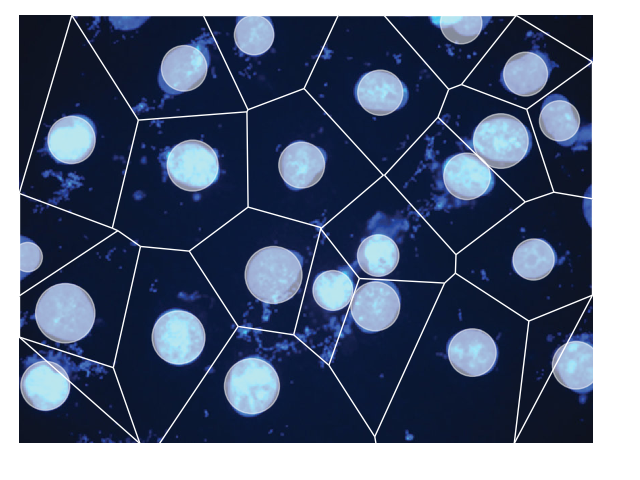
\includegraphics[width=\textwidth]{generators_from_image.png}
	\caption{The opaque circles indicate the generators' location and extent identified by segmentation. The white lines
		indicate Voronoi Tessellation resulting from these generators. Image source: \cite{Folgueras-Flatschart2018}}
\end{figure}

The image segmentation implemented here initially attempts to separate cell nuclei from background followed
by identifying separate individual nuclei and discarding noise to obtain a set of generators matching those displayed in
the image.

Initially, pixels which lie to either side outside of a threshold range of channel
intensity and are assumed to be unambiguously assignable to either background or nuclei are marked.
For flexibility regarding image
brightness, percentiles are employed over static values of channel intensity, i.e. the amount of light.
In the case of the image above the background can be clearly distinguished.

However, as nuclei present a heterogenous texture most accurate results in terms of specificity are achieved when
marking nuclei only by their most intense pixels and employing the Watershed algorithm to extend the selection
to the entire circular region. The algorithm works by filling distinct areas of a topology map.
areas are bounded by edges. A Sobel filter was used for edge detection and the boundaries
of the cell nuclei were reliably identified in the example above.
The final segmentation is determined by borders where distinct areas touch.
Each initial marker determines how the entire area, containing unmarked pixels, is marked.

The cell nuclei can be separated from the background accurately using this approach. However, since two distinct
ranges of channel intensity, i.e. criteria, were employed to place initial markers, only two separate objects exist
initially, one being the background, the other being all nuclei. These may be separated based on connectivity.
As a result, each nucleus is identified by a connected region of non-zero entries in a Numpy array.

Numpy features functionality to determine the extent and centroid of these regions, which further allows to discriminate
noise from a nuclei by size. This parameter requires adjustment to the image. For flexibility, the percentile is employed.

\subsection{Voronoi Tessellations}
A similar approach to the segmentation approach presented in the previous section was employed to
determine a planar graphs embedding from immunofluorescence stained dystrophin in muscle tissue.
Despite not highlighting the cell membrane, the image was employed for development of the segmentation,
due to its clarity and degree of detail.

\begin{figure}[H]
	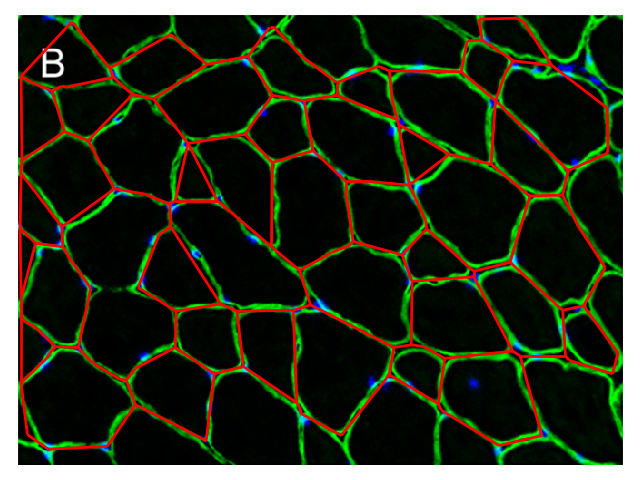
\includegraphics[width=\textwidth]{voronoi_tessellation_from_image.png}
	\caption{The red lines indicate the embedding obtained, implicitly assumed to resemble
		a Voronoi Tessellation. Image source: \cite{Park2015}}
\end{figure}

Similar to the approach previously presented the initial task is to separate dystrophin from the background, which
is achieved by means of channel intensity. By separating the individual regions of the background, it is possible
to filter these spaces by size and discard small regions of background and thereby simplify the structure of
the resulting graph.

After the structure of dystrophin is separated, it is necessary to derive a graph embedding from its individual
branching points and connecting segments. A central problem is the variable width of the structure, preventing
an adjacency based traversal of the pixels, as described in the appendix of \cite{Schneider2015}.
This obstacle is avoided by employing an algorithm for topological skeletonization provided by the scikit-image library.
The algorithm works by removing pixels from the objects border while maintaining connectivity. It thereby creates a
version of the shape reduced to single lines, which are equidistant to the boundaries of the shape, an outline
of the shape.

This results in a thinned representation of the dystrophin structure, in which connecting segments are reduced to a width
of a single pixel. As a result, pixels with more than two adjacent pixels, i.e. branching points, can be
unambiguously identified, which correspond to nodes in a graphs' embedding. By applying a variation of Depth-first search
adapted from \cite{Schneider2015} adjacency relationships between the branching points can be determined and edges
established in the final representation of the graph.

\section{Implementation}
The interface consists of a wrapper implemented in Python and a core program implemented in C++ and is intended
to be used like a Python library. The C++ component computes tessellations, while the Python component supplies parameters,
including generator sets, performs image segmentation and visualization of tessellations.
It also makes additional information on the obtained tessellation accessible, which is,
given the necessity of intensive computations, performed by the C++ component.

\subsection{File formats}
Both components transmit information via temporary files. Generator sets are represented as \texttt{.csv} files,
each line specifying the x-coordinate, y-coordinate and weight of one generator.

Tessellations, being embeddings of graphs, are represented as \texttt{.graphml} files. GraphML is a common XML grammar.

Generators sets as well as Voronoi Tessellations and Delaunay Triangulations may be saved in and loaded from the respective
file formats, tessellations including their associated information.

\subsection{Object structure}
A Python object representing a Voronoi Tessellation contains additional information beyond a graphs embedding
that is employed for visualization. The visualization is facilitated via the NetworkX library, providing
its own graph implementation.

While this component is available to the user, the object also stores specialized representations of graph components
which are native to this library and therefore customizable.

\lstset{style=python_code}
\begin{lstlisting}[language=Python, 
	caption={Python code to output the components of a \texttt{VoronoiTessellation} object}, captionpos=b]
import pprint
from voronoi import voronoi

generators = voronoi.Generators()
generators.randomize(num=5)

voronoi_tessellation = voronoi.VoronoiTessellation()
voronoi_tessellation.compute_from_generators(generators)

pp = pprint.PrettyPrinter(width=60)

print("voronoi_tessellation.nodes:")
pp.pprint(voronoi_tessellation.nodes)
print()

print("voronoi_tessellation.edges:")
pp.pprint(voronoi_tessellation.edges)
print()

print("voronoi_tessellation.faces:")
pp.pprint(voronoi_tessellation.faces)
\end{lstlisting}

The above Python code will produce an output similar to the one below, subject to random generators,
representing the attributes accessible. The indices correspond with the \texttt{.graphml} file generated
by the C++ component.

\lstset{style=output}
\begin{lstlisting}
voronoi_tessellation.nodes:
[{'angles': (2.51657, 1.38737, 2.37924),
  'position': (197.172, 281.079)},
 {'angles': (1.22272, 2.92178, 2.13868),
  'position': (397.295, 448.882)},
 {'angles': (2.31748, 1.94867, 2.01704),
  'position': (394.645, 469.167)},
 {'angles': (3.33899, 0.316959, 2.62724),
  'position': (0.0, 630.0)},
 {'angles': (0.954005, 0.67373, 4.65545),
  'position': (0.0, 749.0)},
 {'angles': (4.51499, 1.3228, 0.445392),
  'position': (126.0, 0.0)},
 {'angles': (4.21365, 0.848445, 1.22109),
  'position': (561.0, 0.0)},
 {'angles': (5.26807, 0.450822, 0.564298),
  'position': (1000.0, 806.0)}]

\end{lstlisting}
\pagebreak
\begin{lstlisting} [caption={The Python representation of a Voronoi Tessellation's attributes as printed by the script above.}, 
	captionpos=b]
voronoi_tessellation.edges:
[{'length': 400.777, 'nodes': {'3', '0'}},
 {'length': 261.164, 'nodes': {'1', '0'}},
 {'length': 289.95, 'nodes': {'5', '0'}},
 {'length': 20.4576, 'nodes': {'1', '2'}},
 {'length': 477.801, 'nodes': {'6', '1'}},
 {'length': 483.788, 'nodes': {'4', '2'}},
 {'length': 692.756, 'nodes': {'7', '2'}},
 {'length': 642.476, 'nodes': {'3', '5'}},
 {'length': 119.0, 'nodes': {'3', '4'}},
 {'length': 1001.62, 'nodes': {'7', '4'}},
 {'length': 435.0, 'nodes': {'6', '5'}},
 {'length': 917.8, 'nodes': {'6', '7'}}]

voronoi_tessellation.faces:
[{'area': 78727.5,
  'centroid': (181.458, 504.876),
  'nodes': ('4', '2', '1', '0', '3')},
 {'area': 40127.1,
  'centroid': (107.724, 303.693),
  'nodes': ('5', '3', '0')},
 {'area': 119786.0,
  'centroid': (339.002, 166.955),
  'nodes': ('6', '5', '0', '1')},
 {'area': 151164.0,
  'centroid': (464.882, 674.722),
  'nodes': ('7', '2', '4')},
 {'area': 171089.0,
  'centroid': (650.63, 424.314),
  'nodes': ('7', '6', '1', '2')}]
\end{lstlisting}

Most attributes should be intuitively denoted. The angles of nodes, however, are determined and represented according to
conventions in the field of force inference. Given a vertex, all \(k\) adjacent edges, representing forces \(F_1, \dots, F_k\),
are sorted in counter-clockwise order. Clockwise angles are determined between the edges. Following the order of edges this
produces an ordered sequence of angles, here represented as tuples. Angles are given in radians.

As edges are undirected, their nodes are stored in sets. Finally, the nodes of a face are ordered according to the faces'
perimeter.

Excluding information on faces, analogous information is available for Delaunay Triangulations.

\subsection{Benchmark}
\begin{figure}[H]
	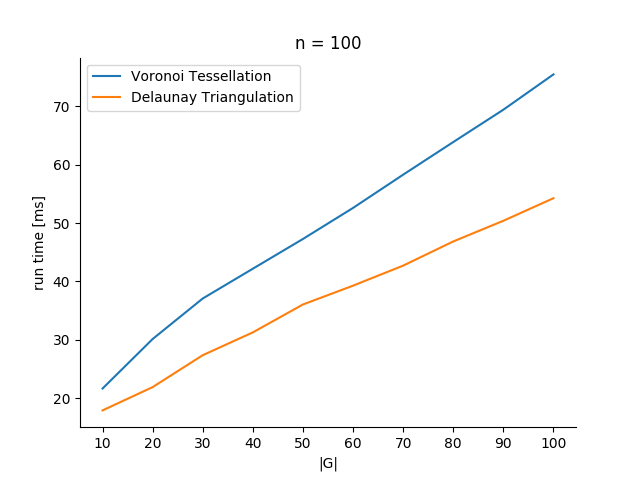
\includegraphics[width=\textwidth]{benchmark.png}
	\caption{The median duration of the creation of a Voronoi Tessellation and Delaunay Triangulation, respectively,
		for variable \(|G|\) sampled from \(n\) runs per generator number.
		The difference between both durations increases visibly in accordance with the above-linear complexity of obtaining
		a Voronoi Tessellation from a Delaunay Triangulation.}
\end{figure}

\subsection{Documentation}
The library is documented in its source code by docstrings following numpydoc conventions. 
The documentation is available at 	

\begin{center}
	\href{https://lucasfein.github.io/voronoi/}{\texttt{https://lucasfein.github.io/voronoi/}}
\end{center}

\printbibliography
\end{document}